\begin{frame}{Functional programming}
  \begin{center}
    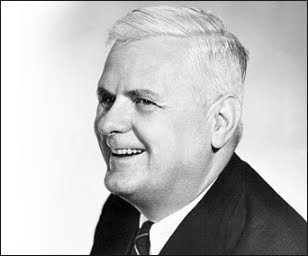
\includegraphics[height=1in]{img/church.jpg}
  \end{center}
  \begin{itemize}
    \item Functional programming is a programming paradigm.
    \item Alonzo Church introduced lambda calculus in 1932:
      $$ \lambda f . ( \lambda x . f ( x x ) ) ( \lambda . f ( x x ) )$$
    \item Church--Turing thesis: lambda calculus \textbf{is} computation.
  \end{itemize}
\end{frame}

\begin{frame}{Imperative programming}
  \begin{center}
    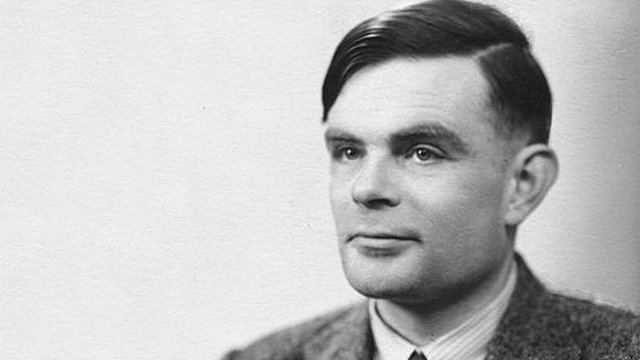
\includegraphics[height=1in]{img/alanturing.jpg}
  \end{center}
  \begin{itemize}
    \item Functional contrasts with imperative programming.
    \item C, Java, JavaScript are largely imperative.
    \item Programs have \textbf{state}, modified by \textbf{statements}.
    \item Origins in the Turing machine, a conceptual model created by Alan Turing.
  \end{itemize}
\end{frame}